\documentclass[]{AVSSimReportMemo}
\usepackage{AVS}
\usepackage{colortbl}

\newcommand{\ModuleName}{singleAxisSpin}
\newcommand{\subject}{Guidance Module to Perform a Spinning about an Arbitrary Axis}
\newcommand{\status}{Initial Version}
\newcommand{\preparer}{M. Cols}
\newcommand{\summary}{Generate the reference attitude trajectory for a general spinning about an arbitrary axis. The spinning is superimposed to a zero reference attitude }


\begin{document}


\makeCover


%
%	enter the revision documentation here
%	to add more lines, copy the table entry and the \hline, and paste after the current entry.
%
\pagestyle{empty}
{\renewcommand{\arraystretch}{2}
\noindent
\begin{longtable}{|p{0.5in}|p{4.5in}|p{1.14in}|}
\hline
{\bfseries Rev}: & {\bfseries Change Description} & {\bfseries By} \\
\hline
Draft & initial copy & M. Cols \\
\hline

\end{longtable}
}

\newpage
\setcounter{page}{1}
\pagestyle{fancy}

\tableofcontents
~\\ \hrule ~\\

\section{Module Input and Output}
Table \ref{tab:inputTable} shows the input Configuration Data of the module Single Axis Spin.
\begin{table}[h!]
	\centering
	\caption{Input Configuration Data}
	\begin{tabular}{|l|l|l|p{3in}|}
		\hline
		\rowcolor{BrickRed}
		\textcolor{white}{Name} & \textcolor{white}{Type} & 
		\textcolor{white}{Length} & 
		\textcolor{white}{Description}  \\ \hline
		$\bm{\sigma}_{R_0/N}$ & double [] & 3 & 
		MRP attitude set of the base reference with respect to the inertial frame . \\ \hline
		$\bm{\omega}_{\textrm{spin}}$& double [] & 3 & 
		Angular velocity of the desired spinning reference with respect to the inertial expressed in inertial frame components. \\ \hline
	\end{tabular}
	\label{tab:inputTable}
\end{table}

Table \ref{tab:outputTable} shows the Attitude Reference output message of the module Single Axis Spin.
\begin{table}[h!]
	\centering
	\caption{Output Attitude Reference Message}
	\begin{tabular}{|l|l|l|p{3in}|}
		\hline
		\rowcolor{BrickRed}
		\textcolor{white}{Name} & \textcolor{white}{Type} & 
		\textcolor{white}{Length} & 
		\textcolor{white}{Description}  \\ \hline
		$\bm{\sigma}_{R/N}$ & double [] & 3 & 
		MRP attitude set of the reference frame with respect to the inertial frame. \\ \hline
		$\leftexp{N} {\bm{\omega}_{R/N}}$ & double [] & 3 & 
		Angular rate vector of the reference frame with respect to the inertial expressed in inertial frame components. \\ \hline
		$\leftexp{N} {\dot{\bm{\omega}}_{R/N}}$ & double [] & 3 & 
		Angular acceleration vector of the reference frame with respect to the inertial expressed in inertial frame components. \\ \hline
	\end{tabular}
	\label{tab:outputTable}
\end{table}
\newpage

\section{Introduction}
This technical note discusses the mathematics to compute a reference frame $\mathcal{R}$ that superimposes a spinning motion, defined by an input angular vector $\bm{\omega}_{\textrm{spin}}$, on top of a zero base reference frame $ \bm{\sigma}_{R_0/N} = [0, 0, 0]$ , as shown in Figure~\ref{fig:fig1}.
\begin{figure}[htb]
	\centerline{
	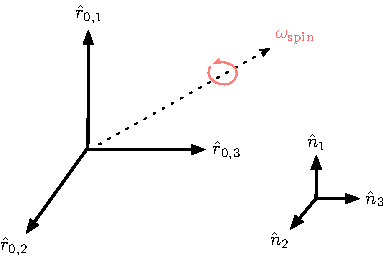
\includegraphics{Figures/fig1}
	}
	\caption{Illustration of the input base frame $\mathcal{R}_{0}:\{ \hat r_{0,1}, \hat r_{0,2}, \hat r_{0,3} \}$,  the inertial frame $\mathcal{N}:\{ \hat{\bm n}_{1}, \hat{\bm n}_{2}, \hat{\bm n}_{3} \}$ and the arbitrary axis about which the spinning is performed at an angular rate  $|\bm{\omega}_{\textrm{spin}}|$. The orientation of the spinning arbitrary axis is determined by the vectorial part of the input angular vector, while the rate correspond to its magnitude.}
	\label{fig:fig1}
\end{figure}

\section{Reference Frame Generation}
Given the inertial nature of the spinning motion, the angular velocity of the desired reference frame is simply the input angular vector $\bm{\omega}_{\textrm{spin}}$. Since the angular rate is assumed to be constant, the angular acceleration is zero.
\begin{equation}
	\leftexp{N} {\bm{\omega}_{R/N}} = \bm{\omega}_{\textrm{spin}}
\end{equation}
\begin{equation}
	 \dot{\bm{\omega}}_{R/N} = 0
\end{equation}
With respect to the initial attitude reference $\mathcal{R}_0$, the orientation of the desired reference $\mathcal{R}$ is defined at each time step through a principal rotation vector:
\begin{equation}
	\hat{\bm{e}}_{\textrm{spin}} = t_{\textrm{mnvr }} \omega_{R/N}
\end{equation}
Where $ t_{\textrm{mnvr }}$ is the time elapsed since the start of the spinning maneuver, after the pointing towards the spinning direction had been stabilized.
The corresponding Direction Cosine Matrix is computed using the following function from the Rigid Body Kinematics library of Reference~\citenum{schaub}:
\begin{equation}
	[C_{\textrm{spin}}] = PRV2C(\hat{\bm{e}})
\end{equation}
The MRP attitude set of the reference $\mathcal{R}$ with respect to the inertial frame $\mathcal{N}$ is then obtained making use of the DCM addition property and several convenient methods from Reference ~\citenum{schaub}:
\begin{equation}
	[R_{0}N] = \textrm{MRP2C}( \bm{\sigma}_{R_{0}N})
\end{equation}
\begin{equation}
	[RN] = [C_{\textrm{spin}}][R_{0}N]
\end{equation}
\begin{equation}
	\bm{\sigma}_{RN} =  \textrm{C2MRP}([RN])
\end{equation}

\bibliographystyle{unsrt}
\bibliography{references}

\end{document}
